\documentclass[10pt,aspectratio=43]{beamer}
\usepackage{fsu2017}
% the aspactratio defines the foramt
% default is 43 (4:3, 128mm:96mm), alternatives are
% 32 (3:2, 135mm:90mm)
% 54 (5:4, 125mm:100mm)
% 149 (14:9, 14cm:9cm)
% 169 (16:9, 16cm:9cm)
% 1610 (16:10, 16cm:10cm)
% 141 (1.41:1, 148.5mm:105mm, ratio of DinA)

\usepackage{color}
\usepackage[backend=biber,style=authoryear]{biblatex} % or any other style you prefer
\addbibresource{references.bib}


% graphic settings
\usepackage{graphicx}
\usepackage{tikz}
\usepackage{pgfplots}
\usepackage{amsmath}
\usepackage{accents}
\usepackage{booktabs}
\usetikzlibrary{arrows.meta, positioning, calc}
\pgfplotsset{compat=1.18}
\newcommand{\myvect}[1]{\accentset{\rightharpoonup}{#1}}

\usetikzlibrary{angles, quotes, shapes, decorations.markings, calc, arrows.meta,3d, shapes.multipart}
% Styles
%% Node Style in Order Text to Get Center Alignment
\tikzset{every text node part/.style={align=center}}
%% Bottom Ray Outside Box
\tikzset{
	every text node part/.style = {align=center},
	rayE2/.style = {
		postaction = decorate,
		decoration = {
			markings,
			mark = at position 0.52 with {\arrow{stealth}}
		}
	}
}

% Custom citation: author + title only
\DeclareCiteCommand{\authortitlefootcite}
{\usebibmacro{prenote}}
{%
	\printnames{labelname}%
	\addcomma\space%
	\printfield[citetitle]{title}%
}
{\multicitedelim}
{\usebibmacro{postnote}}




\title[Parameter estimation]{Parameter estimation\\with correlated photon pairs}
\author[Jan Gößwein]{Jan Gößwein}
\date{Jena, \today}
\institute[IAP]{Institute of Applied Physics}

\begin{document}
	
	%% titlepage
	\showheadlinefalse
	\begin{frame}[noframenumbering]
		\titlepage
	\end{frame}
	
	
	
	
	\showheadlinefalse
	\begin{frame}{Table of content}
		\tableofcontents
	\end{frame}
	
	\showheadlinetrue
	
	\section{Motivation}
		
	\begin{frame}{Motivation}
			% Start a TikZ picture environment
			\begin{center}
				
			
			\begin{tikzpicture}[baseline, node distance=2cm and 2cm]
				
				% Top image
				\node (p)  {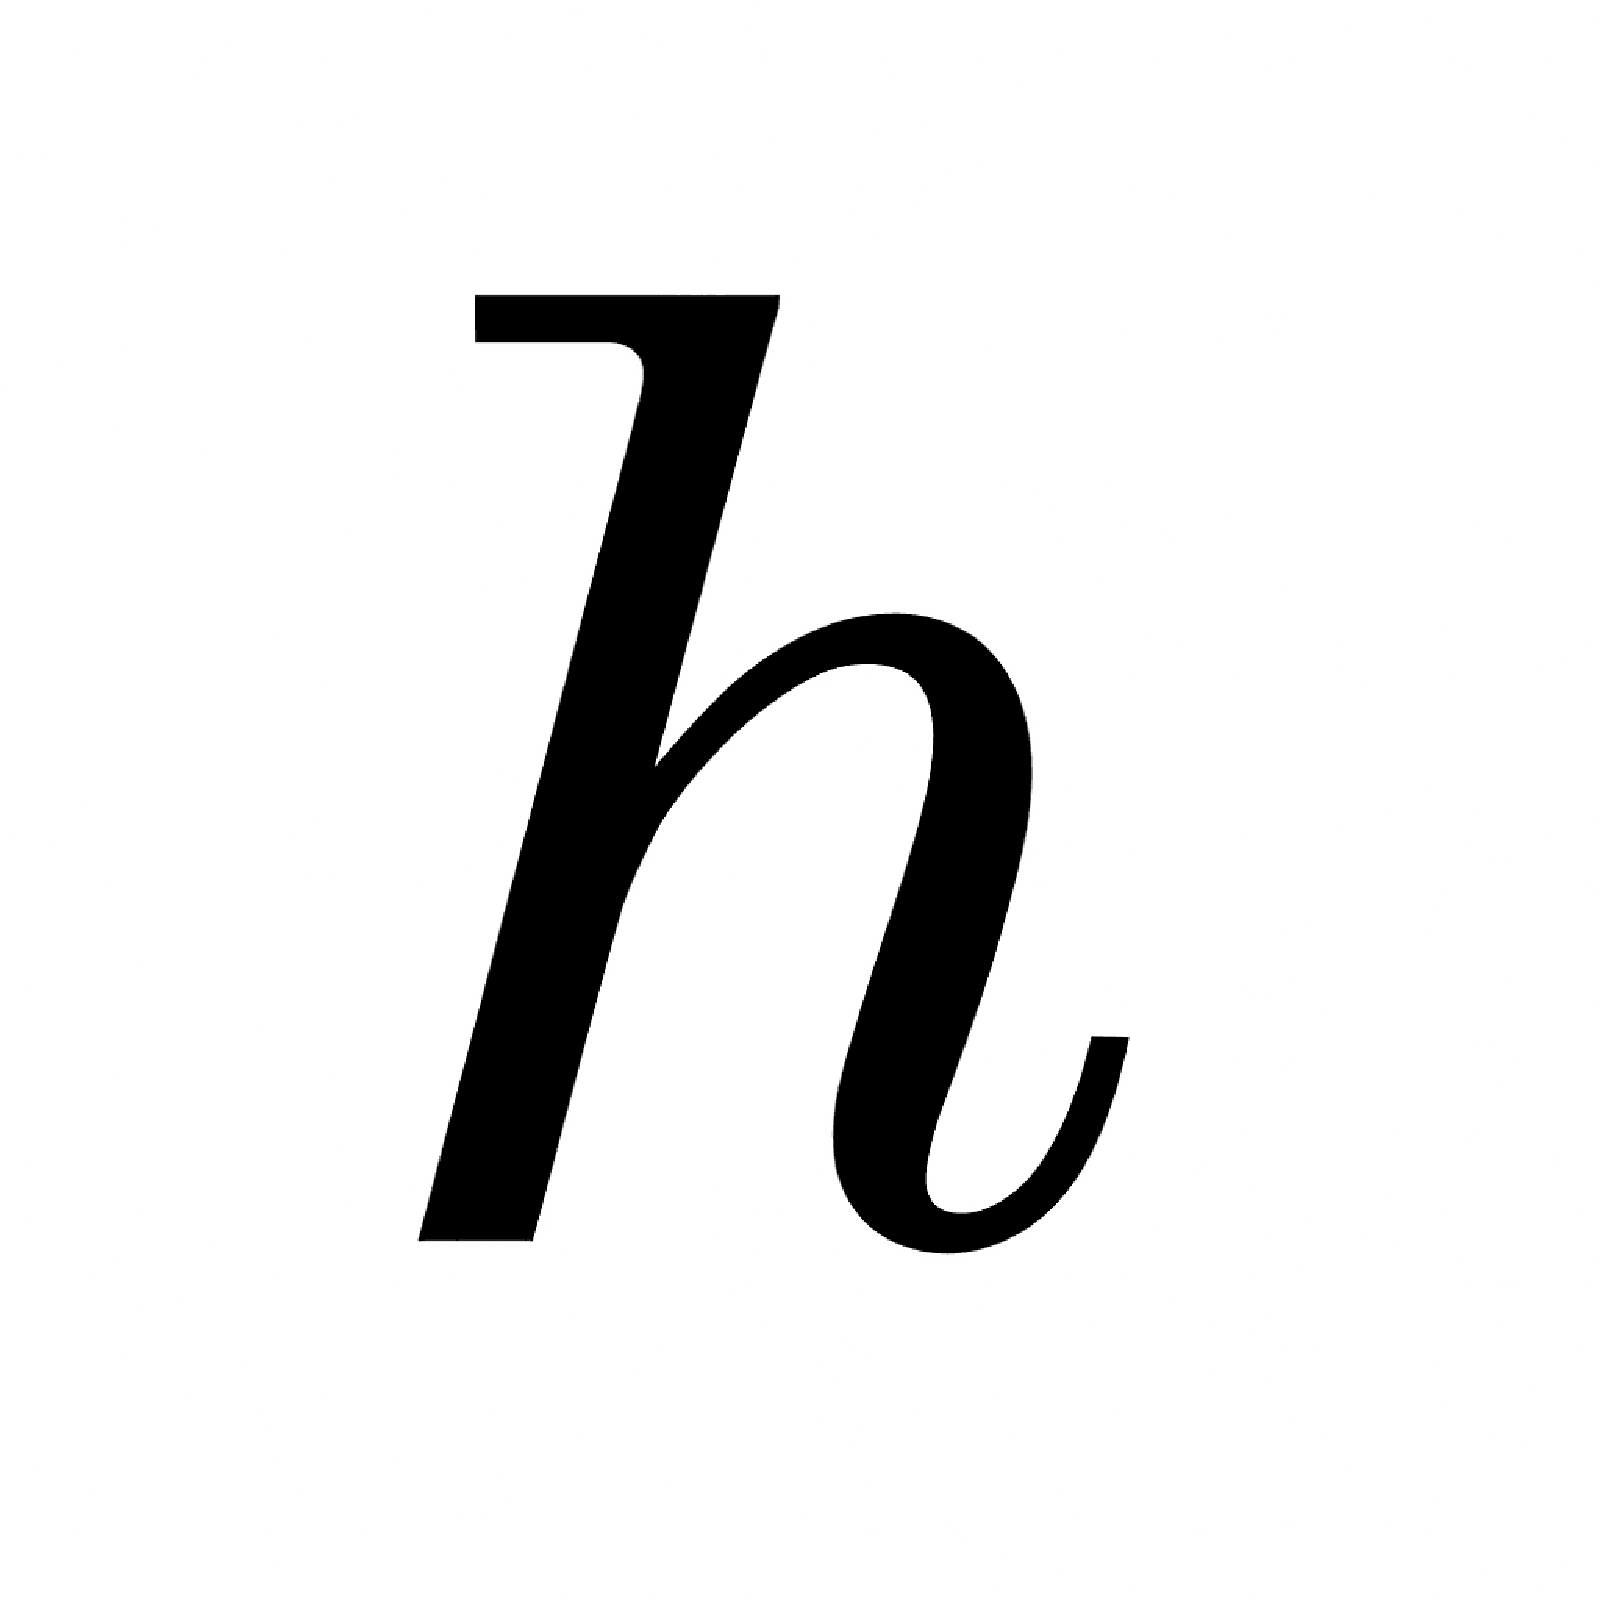
\includegraphics[width=.1\textwidth]{Images/PureImage.pdf}};
				\node (a) [right=of p] {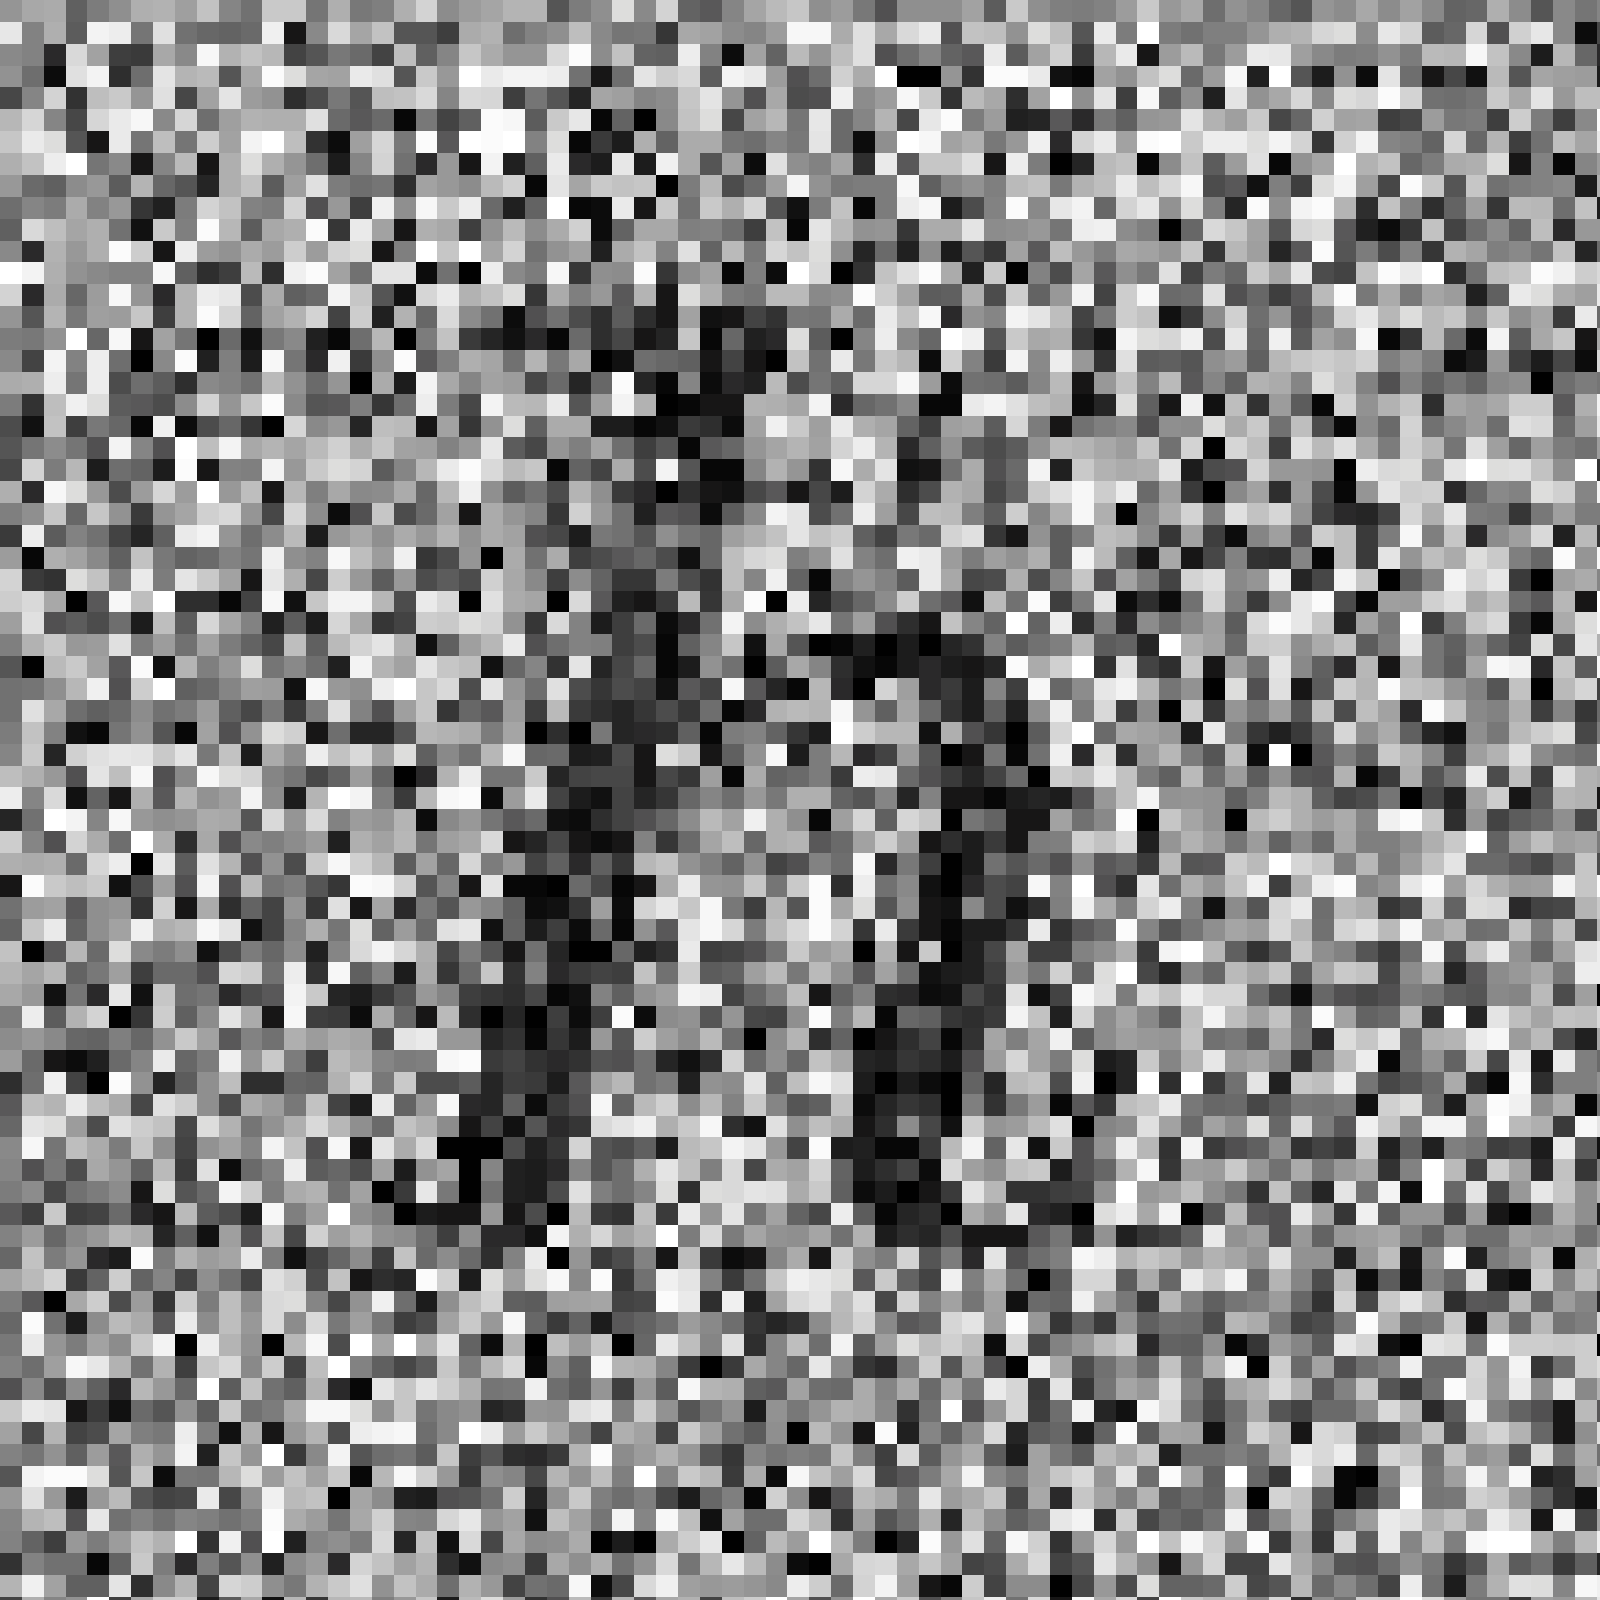
\includegraphics[width=.1\textwidth]{Images/NoisyImage.pdf}};
				% Bottom image
				\node (b) [right=of a] {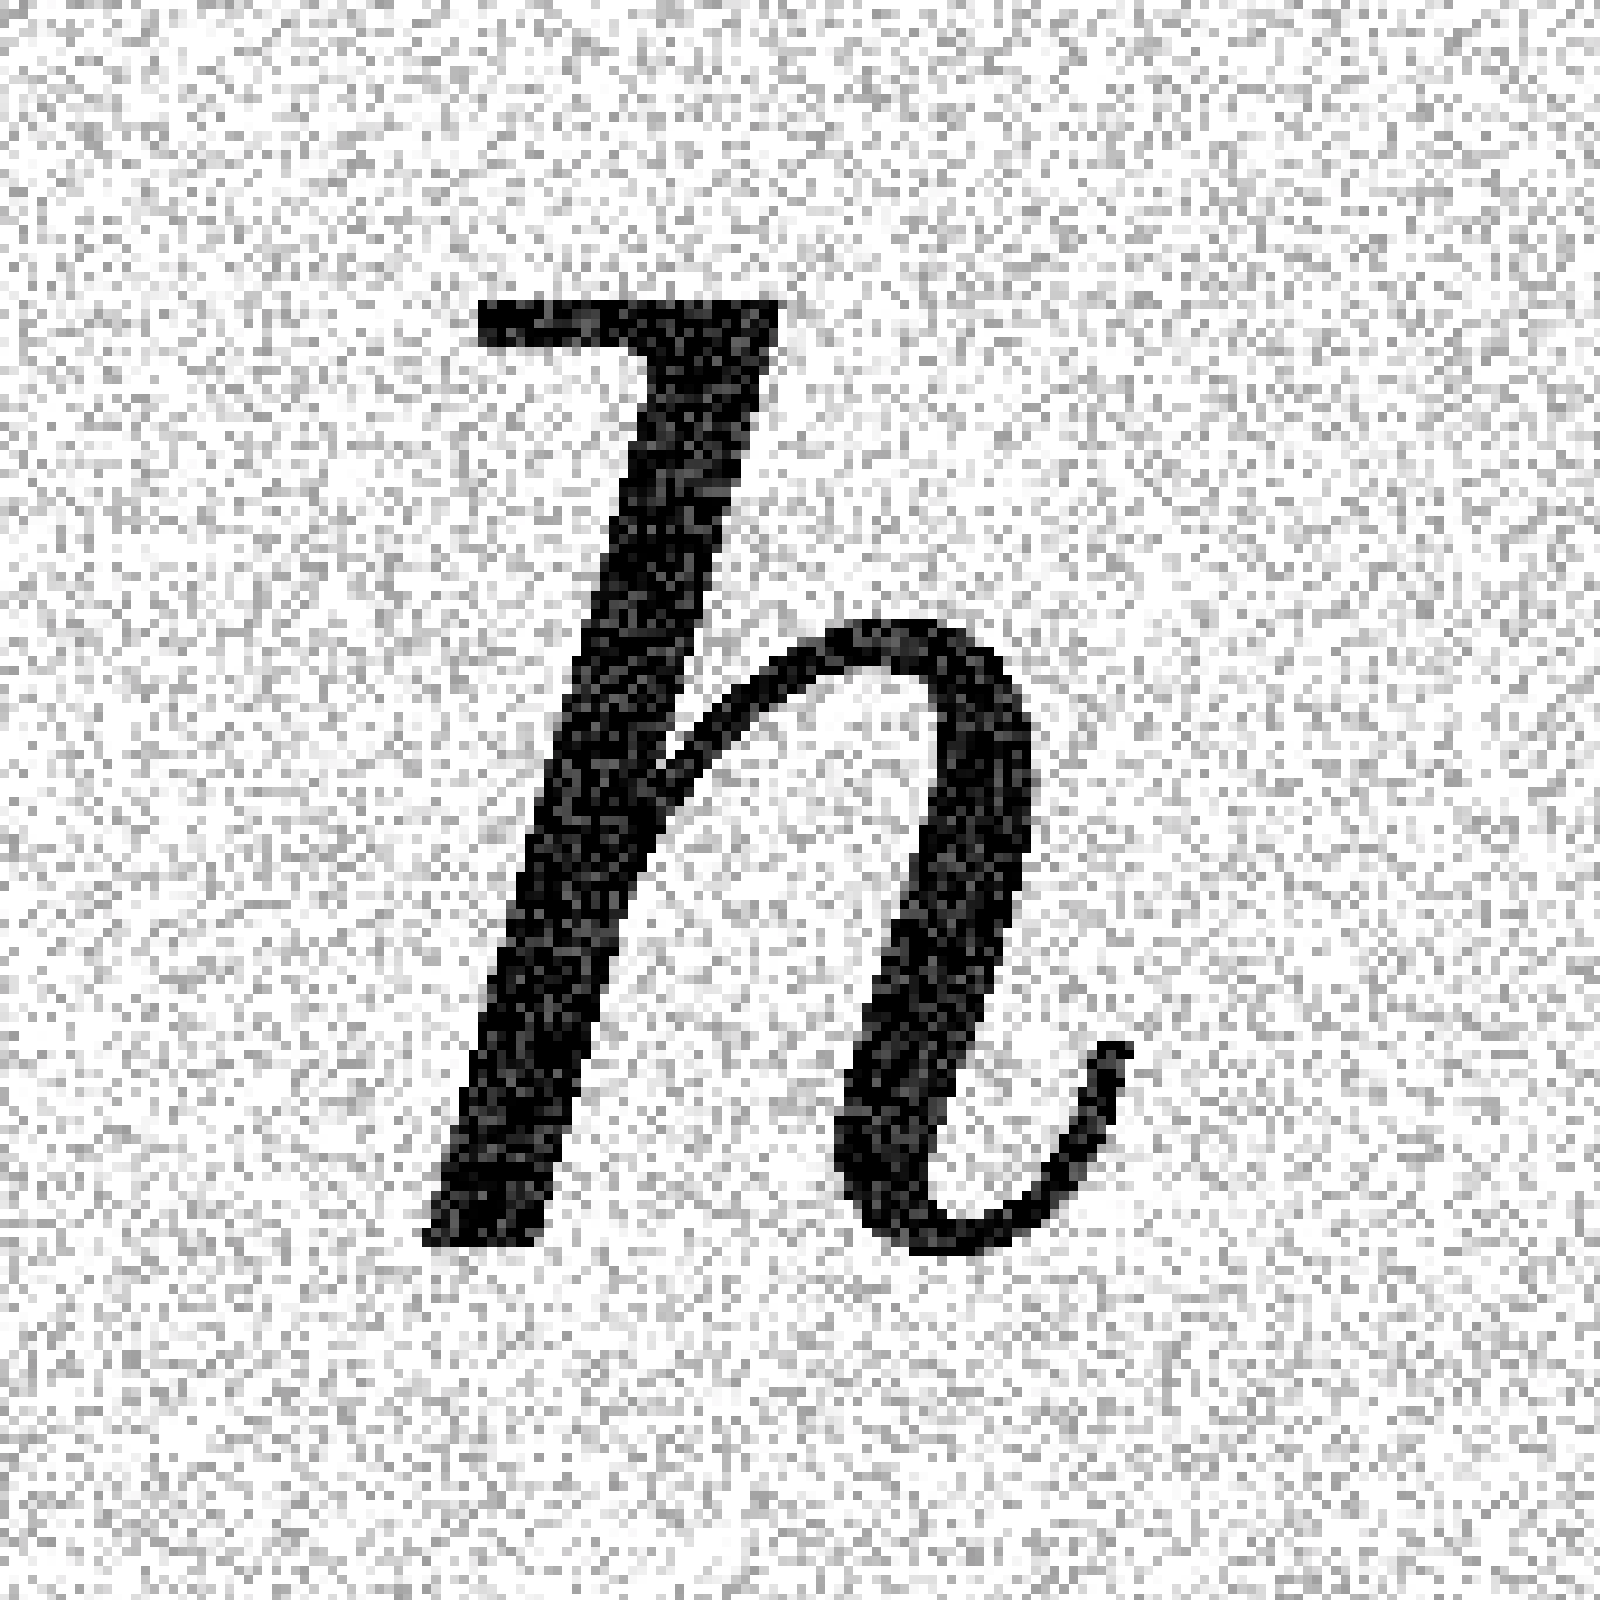
\includegraphics[width=.1\textwidth]{Images/BetterImage.pdf}};
				% Left image, vertically centered between a and b
				
				
				% Arrows
				\draw[-{Latex[length=2mm]}, thick] (p.east) -- node[above] {add noise} (a.west);
				\draw[-{Latex[length=2mm]}, thick] (a.east) to node[above] {$|\phi\rangle$ \footnote{\authortitlefootcite{bridaExperimentalRealizationSubshotnoise2010}}} (b.west);
			\end{tikzpicture}
			\end{center}
			\vspace*{2em}
			\textbf{Objective:} Can correlated photons provide advantages in terms of precision in noisy regimes?
	\end{frame}
	
	\section{Theory}
	
	\begin{frame}{SPDC}
		\visible<2->{
		\begin{minipage}{.45\textwidth}
			\begin{center}
				\resizebox{.7\textwidth}{!}{%
					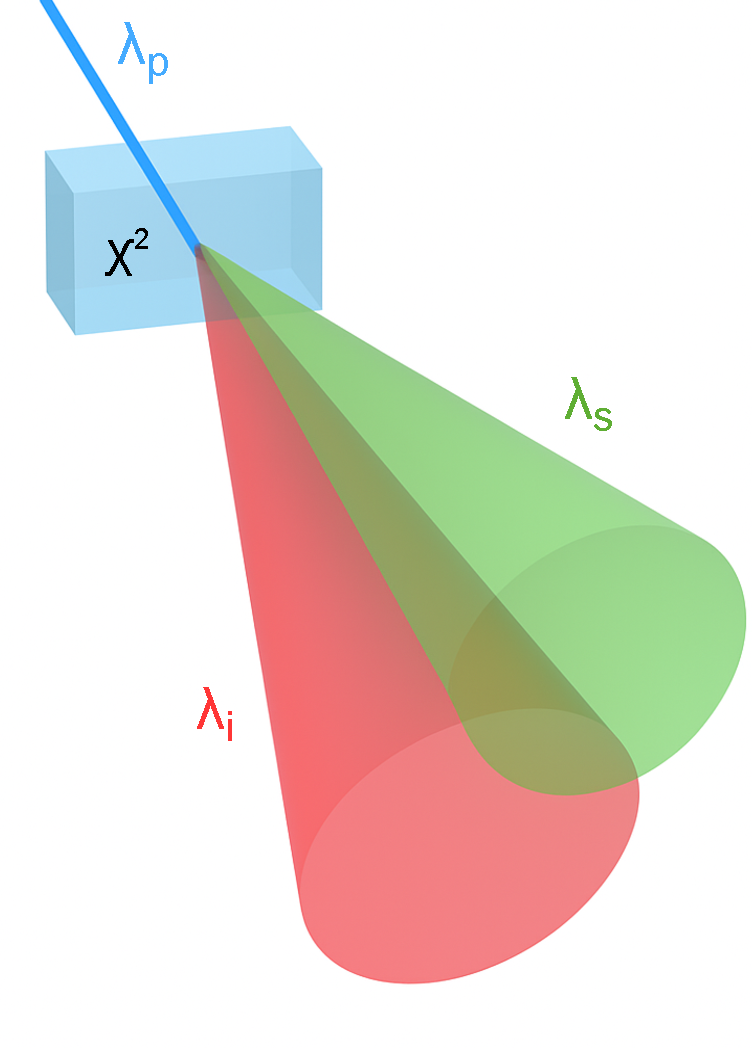
\includegraphics[scale=1]{Images/SPDC_Cone.pdf}
				}%
			\end{center}
		\end{minipage}
		}
%			\begin{minipage}{.45\textwidth}
%			\begin{center}
%				\resizebox{\textwidth}{!}{%
%					\begin{tikzpicture}
%						%\useasboundingbox (0,0) rectangle (10,14);
%						\tikzstyle{every node}=[font=\LARGE]
%						
%						\draw [line width=2.5pt, rayE2,color=blue] (2.5,15.25) -- (6.25,15.25);
%						\draw [line width=2.5pt, rayE2,color=black!40!green] (8.5,15.25) -- (12,16.75);
%						\draw [line width=2.5pt, rayE2,color=red] (8.5,15.25) -- (12,13.75);
%						\draw [ fill=black!10 , line width=1.6pt , rounded corners = 9.0] (6.25,16) rectangle (8.5,14.5);
%						
%						\node at (7.45,15.25) {$\chi^2$};
%						\node at (4.4,15.75) [color=blue] { $\lambda_{\text{p}}$};
%						\node at (10.3,16.8) [color=black!40!green] { $\lambda_{\text{s}}$};
%						\node at (10.3,13.7) [color=red] { $\lambda_{\text{i}}$};
%					\end{tikzpicture}
%				}%
%			\end{center}
%			\end{minipage}
			\hfill
			\begin{minipage}{.45\textwidth}
			\visible<3->{
			\begin{minipage}{.8\textwidth}
				\begin{center}
					\resizebox{\textwidth}{!}{%
						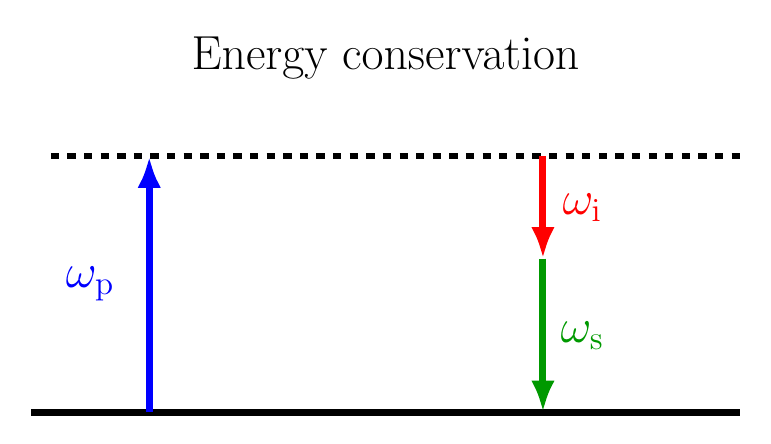
\begin{tikzpicture}
							%\useasboundingbox (0,0) rectangle (10,14);
							\tikzstyle{every node}=[font=\LARGE]
							
							\pgfmathsetmacro{\yTop}{12.5}
							\pgfmathsetmacro{\yBottom}{9.25}
							\pgfmathsetmacro{\yMid}{\yBottom + 0.6*(\yTop - \yBottom)}
							\pgfmathsetmacro{\pLab}{\yBottom + 0.5*(\yTop - \yBottom)}
							\pgfmathsetmacro{\sLab}{\yBottom + 0.3*(\yTop - \yBottom)}
							\pgfmathsetmacro{\iLab}{\yBottom + 0.8*(\yTop - \yBottom)}
							
							
							\draw [line width=2.5pt] (3.5,\yBottom) -- (12.5,\yBottom);
							\draw [ color={rgb,255:red,0; green,0; blue,255}, line width=2.5pt,-{Latex[length=4mm]}] (5,\yBottom) -- (5,\yTop);
							\draw [line width=2.3pt, dashed] (3.75,\yTop) -- (12.5,\yTop);
							\draw [ color={rgb,255:red,255; green,0; blue,0}, line width=2.5pt,-{Latex[length=4mm]}] (10,\yTop) -- (10,\yMid);
							\draw [ color=black!40!green, line width=2.5pt,-{Latex[length=4mm]}] (10,\yMid) -- (10,\yBottom);
							\node [font=\LARGE, color={rgb,255:red,0; green,0; blue,255}] at (4.25,\pLab) {$\omega_{\text{p}}$};
							\node [font=\LARGE, color={rgb,255:red,255; green,0; blue,0}] at (10.5,\iLab) {$\omega_{\text{i}}$};
							\node [font=\LARGE, color=black!40!green] at (10.5,\sLab) {$\omega_{\text{s}}$};
							
							\node [font=\LARGE] at (8,13.75) {Energy\,\,conservation};
							
						\end{tikzpicture}
					}%
				\end{center}
				%\vspace[2em]
				{\footnotesize
					\[
						\omega_{\text{p}} = \omega_{\text{s}} + \omega_{\text{i}}
					\]
				}
			\end{minipage}
			}
			\visible<4->{
			\begin{minipage}{.8\textwidth}
				\vspace*{1.5em}
				\begin{center}
					\resizebox{\textwidth}{!}{%
						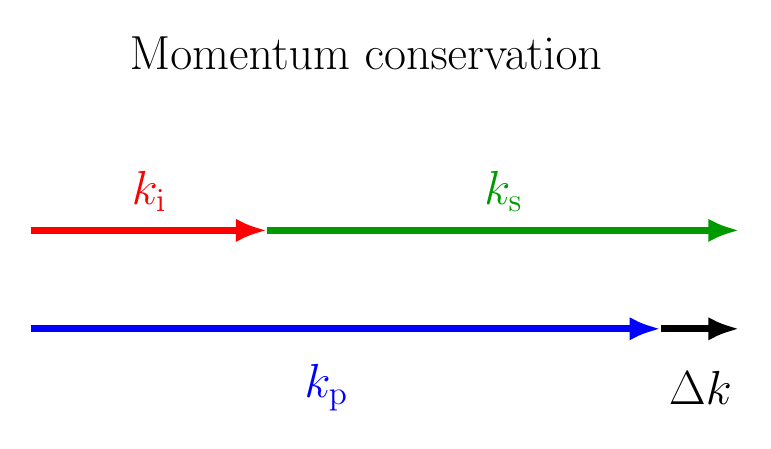
\begin{tikzpicture}
							
							%\useasboundingbox (0,0) rectangle (10,14);
							\tikzstyle{every node}=[font=\LARGE]
							\draw [ color={rgb,255:red,0; green,0; blue,255}, line 	width=2.5pt, -{Latex[length=4mm]}] (15,10.25) -- (23,10.25);
							\draw [ color={rgb,255:red,0; green,0; blue,0}, line width=2.5pt, 	-{Latex[length=4mm]}] (23,10.25) -- (24,10.25);
							\draw [ color={rgb,255:red,255; green,0; blue,0}, line 	width=2.5pt, -{Latex[length=4mm]}] (15,11.5) -- (18,11.5);
							\draw [ color=black!40!green, line width=2.5pt, 	-{Latex[length=4mm]}] (18,11.5) -- (24,11.5);
							
							\node [font=\LARGE, color={rgb,255:red,0; green,0; blue,255}] at 	(18.75,9.5) {$k_{\text{p}}$};
							\node [font=\LARGE, color={rgb,255:red,0; green,0; blue,0}] at 	(23.5,9.5) {$\Delta k$};
							\node [font=\LARGE, color={rgb,255:red,255; green,0; blue,0}] at 	(16.5,12) {$k_{\text{i}}$};
							\node [font=\LARGE, color=black!40!green] at (21,12) 	{$k_{\text{s}}$};
							\node [font=\LARGE] at (19.25,13.75) {Momentum\,\,conservation};
						\end{tikzpicture}
						 
					}%
				\end{center}
				%\vspace[2em]
				{\footnotesize
					\[
					\myvect{k}_{\text{p}} = \myvect{k}_{\text{s}} + \myvect{k}_{\text{i}} - \Delta \myvect{k}
					\]
				}
			\end{minipage}
			}
			\end{minipage}
	\end{frame}


	\begin{frame}{Parameter estimation}
		\visible<1->{\textbf{Setup:} Transmission setup}\\
		\visible<2->{\textbf{Parameter:} Transmittance $T$}\\
		\visible<3->{\textbf{Estimator:} $\operatorname{Var}(T)$} \vspace*{2em}
		
		\visible<4->{
		\begin{minipage}{.4\textwidth}
			\centering
			Conventional approach:\vspace*{1em}
			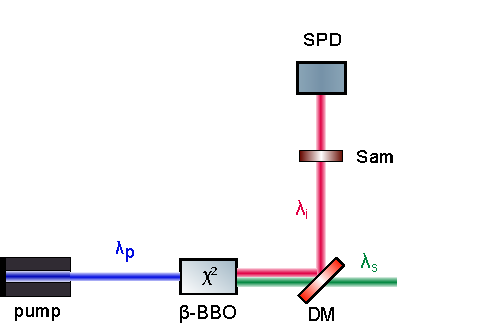
\includegraphics[width=.8\textwidth]{Images/ConventionalSetup.pdf}
		\end{minipage}
		}
		\hfill
		\visible<5->{
		\begin{minipage}{.4\textwidth}
			\centering
			Coincidence approach:\vspace*{1.3em}
			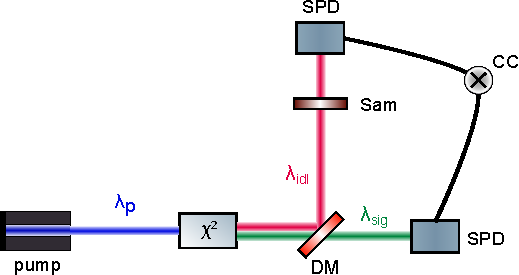
\includegraphics[width=\textwidth]{Images/CoincSetup_Sam.pdf}
		\end{minipage}
		}
	\end{frame}
	
	\begin{frame}{Conventional approach}
		\begin{minipage}{0.6\textwidth}
			\centering
			\only<1>{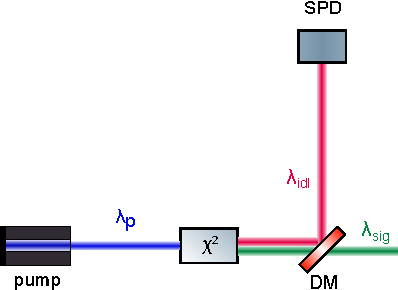
\includegraphics[width=.7\textwidth]{Images/ConventionalSetup_NoSam.pdf}}
			\only<2->{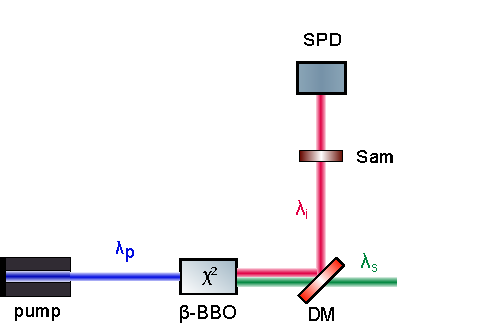
\includegraphics[width=.7\textwidth]{Images/ConventionalSetup.pdf}}
		\end{minipage}%
		\hfill
		\begin{minipage}{0.35\textwidth}
			\[
			\begin{aligned}
				\uncover<1->{N_{\text{tot}}^{\text{ref}} &= \eta_{\text{idl}} N_{\mathrm{g}} + N_{\text{noise}}^{\text{ref}}} \\[0.5em]
				\uncover<2->{N_{\text{tot}}^{\text{sam}} &= T\,\eta_{\text{idl}} N_{\mathrm{g}} + N_{\text{noise}}^{\text{sam}} } \\[1em]
				\uncover<3->{\Rightarrow T &= \frac{\,N_{\text{tot}}^{\text{sam}} - N_{\text{noise}}^{\text{sam}}\,}
				{\,N_{\text{tot}}^{\text{ref}} - N_{\text{noise}}^{\text{ref}}\,} }
			\end{aligned}
			\]
		\end{minipage}
	\end{frame}
		
	
	\begin{frame}{Coincidence approach}
		\begin{minipage}{.6\textwidth}
			\centering
			\only<1>{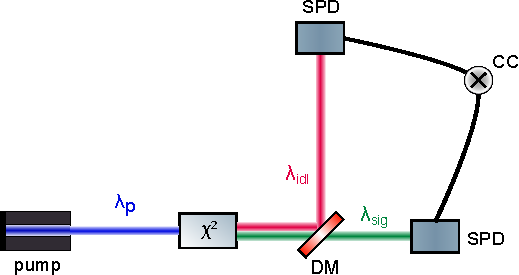
\includegraphics[width=.9\textwidth]{Images/CoincSetup_NoSam.pdf}}
			\only<2->{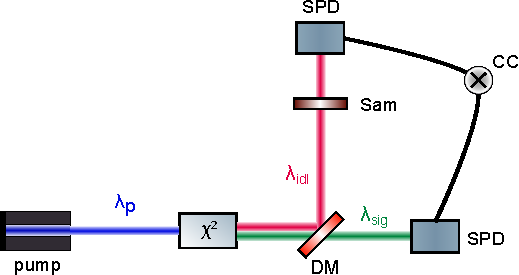
\includegraphics[width=.9\textwidth]{Images/CoincSetup_Sam.pdf}}
		\end{minipage}
		\hfill
		\begin{minipage}{.35\textwidth}
			\[
			\begin{aligned}
				\uncover<1->{N_{\text{cc,tot}}^{\text{ref}} &= \eta_{\text{idl}} \,\eta_{\text{sig}} \, N_{\mathrm{g}} + N_{\text{ac}}^{\text{ref}} } \\[1em]
				\uncover<2->{N_{\text{cc,tot}}^{\text{sam}} &= T \,\eta_{\text{idl}} \,\eta_{\text{sig}} \, N_{\mathrm{g}} + N_{\text{ac}}^{\text{sam}} } \\[1em]
				\uncover<3->{
				\Rightarrow T &= \frac{\,N_{\text{tot,cc}}^{\text{sam}} - N_{\text{ac}}^{\text{sam}}\,}{\,N_{\text{tot,cc}}^{\text{ref}} - N_{\text{ac}}^{\text{ref}}\,}
				} 
			\end{aligned}
			\]
		\end{minipage}
	\end{frame}
	
%	\begin{aligned}
%		\uncover<1->{N_{\text{cc,pure}}^{\text{ref}} &= \eta_{\text{idl}} \,\eta_{\text{sig}} \, N_{\mathrm{g}} \\[0.5em]
%			N_{\text{cc,tot}}^{\text{ref}} &= N_{\text{cc,pure}}^{\text{ref}} + N_{\text{ac}}^{\text{ref}} } \\[1em]
%		\uncover<2->{N_{\text{cc,pure}}^{\text{sam}} &= T \,\eta_{\text{idl}} \,\eta_{\text{sig}} \, N_{\mathrm{g}} \\[0.5em]
%			N_{\text{cc,tot}}^{\text{sam}} &= N_{\text{cc,pure}}^{\text{sam}} + N_{\text{ac}}^{\text{sam}} } \\[1em]
%		\uncover<3->{
%			\Rightarrow T &= \frac{\,N_{\text{tot,cc}}^{\text{sam}} - N_{\text{ac}}^{\text{sam}}\,}{\,N_{\text{tot,cc}}^{\text{ref}} - N_{\text{ac}}^{\text{ref}}\,}
%		} 
%	\end{aligned}
	
	\begin{frame}{Transmittance model}
		\begin{Block}{Conventional approach:}
			\vspace{0.5em}
			\resizebox{\textwidth}{!}{$
				\operatorname{Var}(T) 
				= \left( \eta_{\text{idl}}\,N_{\mathrm{g}} \right)^{-2}
				\Bigg[
				\textcolor<2->{red}{\operatorname{Var}\!\left(N_{\text{tot}}^{\text{sam}}\right)} 
				+ \textcolor<2->{red}{\operatorname{Var}\!\left(N_{\text{noise}}^{\text{sam}}\right)} 
				+ T^{2} \Big[ 
				\textcolor<2->{red}{\operatorname{Var}\!\left(N_{\text{tot}}^{\text{ref}}\right)} 
				+ \textcolor<2->{red}{\operatorname{Var}\!\left(N_{\text{noise}}^{\text{ref}}\right) }
				\Big]
				\Bigg]
			$}
		\end{Block}
		\vspace*{2em}
		\begin{Block}{Coincidence approach:}
			\vspace{0.5em}
			\resizebox{\textwidth}{!}{$
				\operatorname{Var}(T) 
				= \left( \eta_{\text{sig}}\,\eta_{\text{idl}}\,N_{\mathrm{g}} \right)^{-2}
				\Bigg[
				\textcolor<2>{red}{\operatorname{Var}\!\left(N_{\text{tot,cc}}^{\text{sam}}\right) }
				+ \textcolor<2>{red}{\operatorname{Var}\!\left(N_{\text{ac}}^{\text{sam}}\right) }
				+ T^{2} \Big[ 
				\textcolor<2>{red}{\operatorname{Var}\!\left(N_{\text{tot,cc}}^{\text{ref}}\right) }
				+ \textcolor<2>{red}{\operatorname{Var}\!\left(N_{\text{ac}}^{\text{ref}}\right) }
				\Big]
				\Bigg]
			$}
		\end{Block}
	\end{frame}
%	\begin{frame}{Photon statistics}
%		\begin{minipage}{.3\textwidth}
%			\visible<2->{
%			\begin{tikzpicture}
%				\begin{axis}[
%					width=1.2\linewidth,
%					height=1.4\linewidth,
%					xlabel={$n\,\,[a.u.]$},
%					ylabel={$\mathcal{P}(n)\,\,[a.u.]$},
%					xticklabels={},
%					yticklabels={},
%					%grid=major,
%					scaled y ticks = false,
%					tick label style={font=\small},
%					label style={font=\small},
%					legend style={font=\tiny,
%						draw=none,      
%						fill=none,  },
%					]
%					\only<2->{
%					\addplot [mark=none, color=blue, very thick] 
%					table [x index=0, y index=1, header=false] {Images/photon_distributions.txt};
%					\addlegendentry{Poisson}
%					}
%					
%					\only<3->{
%					\addplot [mark=none, color=black, very thick] 
%					table [x index=0, y index=2, header=false] {Images/photon_distributions.txt};
%					\addlegendentry{mmBE}
%					}
%				\end{axis}
%			\end{tikzpicture}
%			}
%		\end{minipage}
%		\hfill
%		\begin{minipage}{.65\textwidth}
%			\visible<2->{
%			Poisson distribution (coherent light): %\footnote{\fullcite{kimPhotoncountingStatisticsbasedSupport2022,schneelochIntroductionAbsoluteBrightness2019}}
%			\[
%			\begin{aligned}
%				\mathcal{P}(n) &= \frac{\langle n\rangle^{n}}{n!}\,e^{-\langle n\rangle} \\ \vspace{5em}
%				\operatorname{Var}(n) &= \langle n\rangle
%			\end{aligned}
%			\]
%			}
%			\visible<3->{
%			multi-mode Bose-Einstein distribution:
%			\[
%			\begin{aligned}
%				\mathcal{P}_m(n) &= \frac{(n+m-1)!}{(m-1)!\,n!}\,
%				\frac{m^m\langle n\rangle^{n}}{\left(m+\langle n\rangle\right)^{n+m}} \\ \vspace{5em}
%				\operatorname{Var}(n) &= \langle n\rangle \left(1+\frac{\langle n\rangle}{m}\right)
%			\end{aligned}
%			\]
%			}
%		\end{minipage}
%	\end{frame}
	
		\begin{frame}{Photon statistics}

			\visible<2->{
				Poisson distribution (coherent light): \footnote<3->{\authortitlefootcite{kimPhotoncountingStatisticsbasedSupport2022}}\footnote<3->{\authortitlefootcite{foucheDetectionFalsealarmProbabilities2003}} 
				\[
				\begin{aligned}
					\mathcal{P}(n) &= \frac{\langle n\rangle^{n}}{n!}\,e^{-\langle n\rangle} \\ \vspace{5em}
					\operatorname{Var}(n) &= \langle n\rangle
				\end{aligned}
				\]
			}
			\visible<4->{
				multi-mode Bose-Einstein distribution (thermal light): \footnotemark[2]
				\[
				\begin{aligned}
					\mathcal{P}_m(n) &= \frac{(n+m-1)!}{(m-1)!\,n!}\,
					\frac{m^m\langle n\rangle^{n}}{\left(m+\langle n\rangle\right)^{n+m}} \\ \vspace{5em}
					\operatorname{Var}(n) &= \langle n\rangle \left(1+\frac{\langle n\rangle}{m}\right)
				\end{aligned}
				\]
			}

	\end{frame}
	
	\section{Experiment}
	\begin{frame}{Experimental setup}
			\begin{center}
				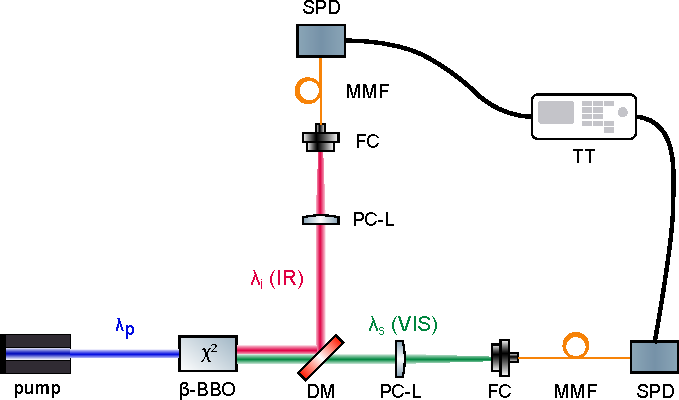
\includegraphics[width=.7\textwidth]{Images/DupishSetupNew.pdf}
			\end{center}
			
	\end{frame}
	
	
	\section{Results}
	
	\begin{frame}{Dark counts}
		\visible<2->{
		\begin{minipage}{.45\textwidth}
			\centering
			Signal arm
			%\vspace{2em}
			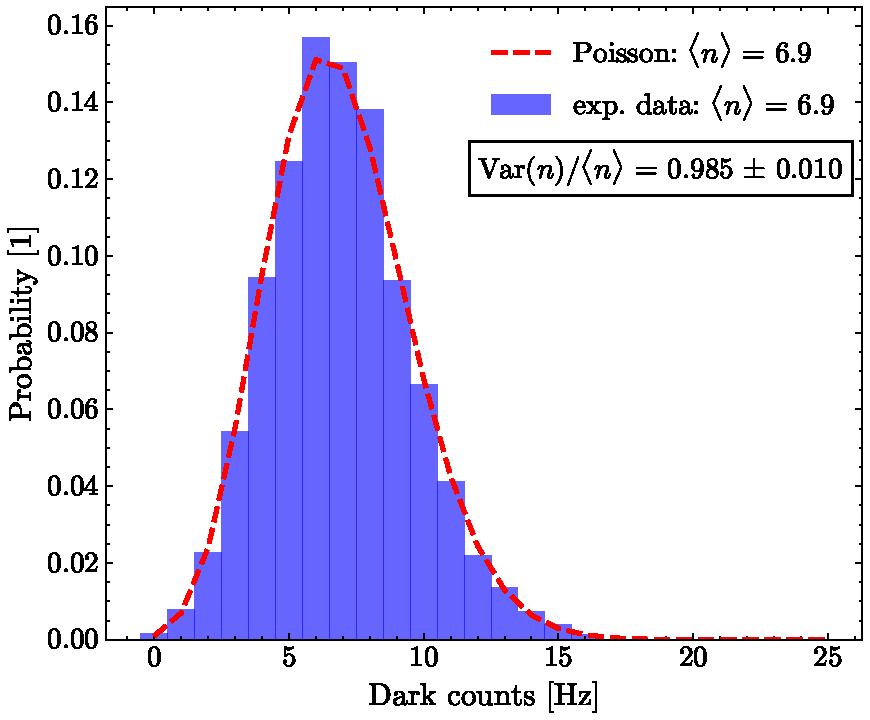
\includegraphics[width=\textwidth]{Images/DC_Sig_2.pdf}
		\end{minipage}
		}
		\hfill
		\visible<3->{
		\raisebox{-2em}{
		\begin{minipage}{.45\textwidth}
			\centering
			Idler arm
			%\vspace{-1.6em}
			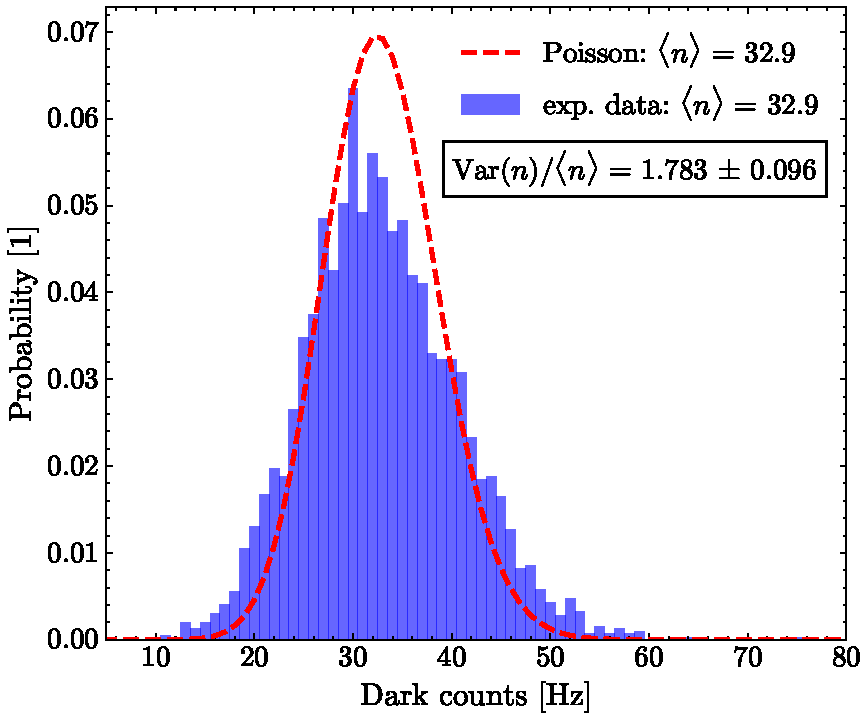
\includegraphics[width=\textwidth]{Images/DC_Idl_2.pdf}
			\visible<4->{
				%\vspace*{1em}
			{\footnotesize
				\[
				\operatorname{Var}\!\left(N_{\text{noise}}\right) = 1.8 \cdot \langle N_{\text{noise}} \rangle
				\]
			}
			}
		
		\end{minipage}
		}
		}
	\end{frame}
	
	\begin{frame}{Single counts}
		\visible<2->{
		\begin{minipage}{.45\textwidth}
			\centering
			Signal arm
			%\vspace*{-1em}
			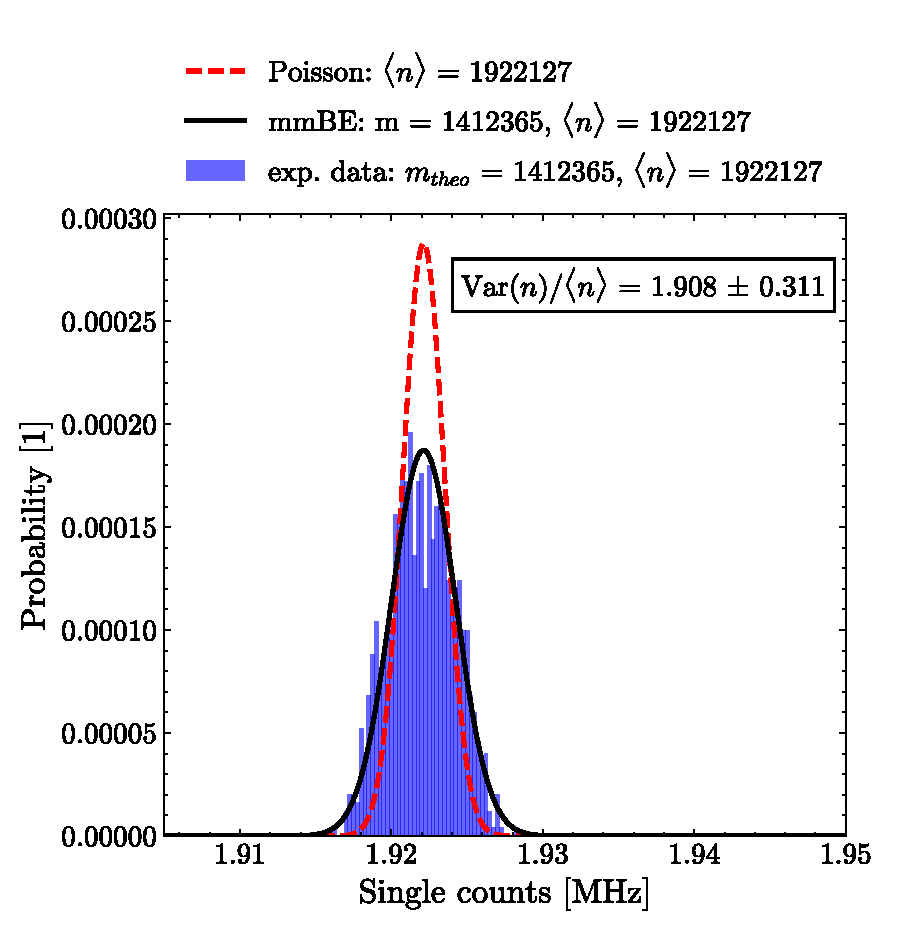
\includegraphics[width=\textwidth]{Images/SingleStatisticsSignal_4.pdf}
		\end{minipage}
		}
		\hfill
		\visible<3->{
			\raisebox{-1em}{
		\begin{minipage}{.45\textwidth}
			\centering
			Idler arm
			%\vspace{2em}
			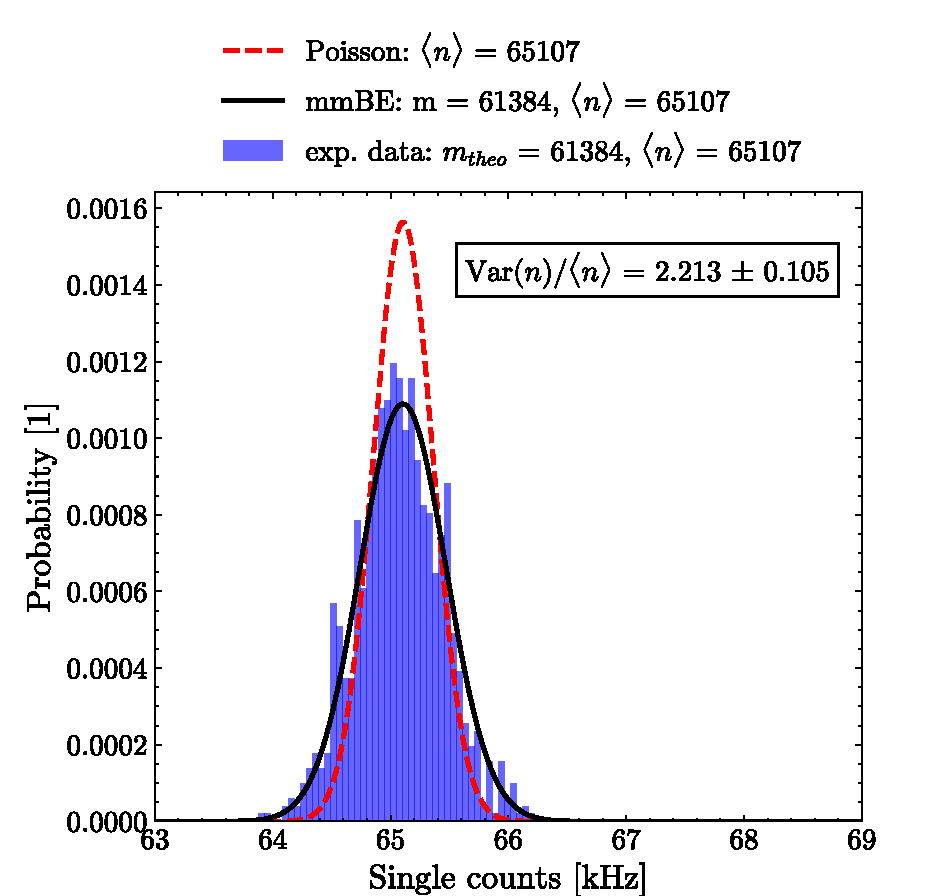
\includegraphics[width=\textwidth]{Images/SingleStatisticsIdler_4.pdf}
			%\vspace*{-2em}
			\visible<4->{
			{\footnotesize
				\[
				\operatorname{Var}\!\left(N_{\text{noise}}\right) = 2.2 \cdot \langle N_{\text{noise}} \rangle
				\]
			}
			}
		\end{minipage}
			}
		}
	\end{frame}
	
	\begin{frame}{Coincidence counts}
		\visible<2->{
		\begin{minipage}{.45\textwidth}
			\centering
			Coincidences
			\vspace{2em}
			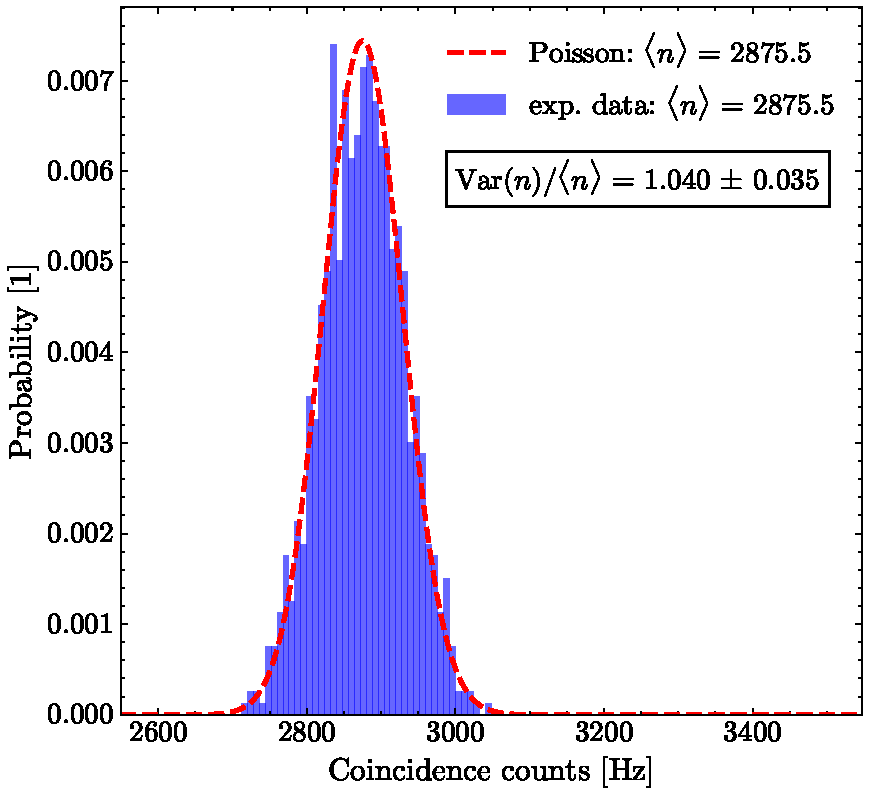
\includegraphics[width=\textwidth]{Images/CoincStatistics_2.pdf}
			\vspace*{-2.5em}
			\visible<3->{
			{\footnotesize
				\[
				\operatorname{Var}\!\left(N_{\text{cc}}\right) = \langle N_{\text{cc}} \rangle
			\]
			}
			}
		\end{minipage}
		}
		\hfill
		\visible<4->{
		\begin{minipage}{.45\textwidth}
			\centering
			Accidentals
			\vspace{2em}
			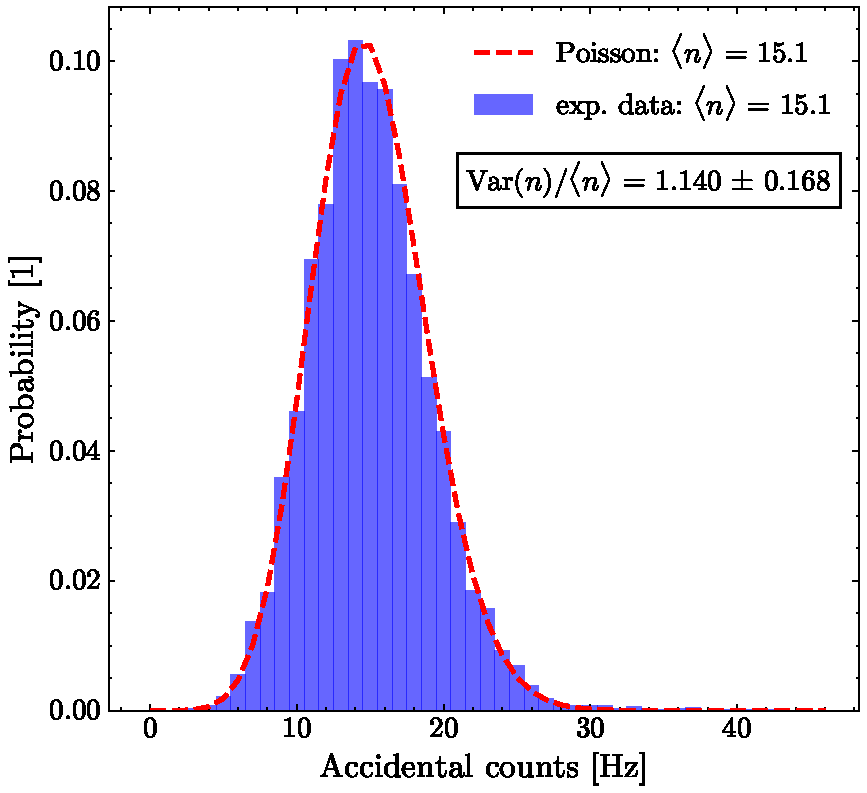
\includegraphics[width=\textwidth]{Images/AccCountsStatistics_2.pdf}
			\vspace*{-2.5em}
			\visible<5->{
				{\footnotesize
					\[
				\operatorname{Var}\!\left(N_{\text{ac}}\right) = \langle N_{\text{ac}} \rangle
			\]
			}
			}
		\end{minipage}
		}
	\end{frame}
	
	
	\section{Simulation}
	\begin{frame}{Simulation}
		\begin{Block}{Conventional approach:}
			\vspace{0.5em}
			\only<1>{
				\resizebox{\textwidth}{!}{$
					\operatorname{Var}(T) 
					= \left( \eta_{\text{idl}}\,N_{\mathrm{g}} \right)^{-2}
					\Bigg[
					\operatorname{Var}\!\left(N_{\text{tot}}^{\text{sam}}\right)
					+ \operatorname{Var}\!\left(N_{\text{noise}}^{\text{sam}}\right)
					+ T^{2}\Big[
					\operatorname{Var}\!\left(N_{\text{tot}}^{\text{ref}}\right)
					+ \operatorname{Var}\!\left(N_{\text{noise}}^{\text{ref}}\right)
					\Big]
					\Bigg]
					$}
			}
			
			% version with <N>
			\only<2->{%
				\resizebox{\textwidth}{!}{$
					\operatorname{Var}(T) 
					= \left( \eta_{\text{idl}}\,N_{\mathrm{g}} \right)^{-2}
					\Bigg[\textcolor{red}{2.2\cdot
					\langle N_{\text{tot}}^{\text{sam}}\rangle}
					+ \textcolor{red}{1.8\cdot\langle N_{\text{noise}}^{\text{sam}}\rangle}
					+ T^{2}\Big[
					\textcolor{red}{2.2\cdot\langle N_{\text{tot}}^{\text{ref}}\rangle}
					+ \textcolor{red}{1.8\cdot\langle N_{\text{noise}}^{\text{ref}}\rangle}
					\Big]
					\Bigg]
					$}
			}
		\end{Block}
		

		\vspace*{2em}
		\visible<3->{
		\begin{Block}{Coincidence approach:}
			\vspace{0.5em}
			\only<3>{
				\resizebox{\textwidth}{!}{$
					\operatorname{Var}(T) 
					= \left( \eta_{\text{sig}}\,\eta_{\text{idl}}\,N_{\mathrm{g}} \right)^{-2}
					\Bigg[
					\operatorname{Var}\!\left(N_{\text{tot,cc}}^{\text{sam}}\right)
					+ \operatorname{Var}\!\left(N_{\text{ac}}^{\text{sam}}\right) 
					+ T^{2} \Big[ 
				\operatorname{Var}\!\left(N_{\text{tot,cc}}^{\text{ref}}\right) 
					+ \operatorname{Var}\!\left(N_{\text{ac}}^{\text{ref}}\right) 
					\Big]
					\Bigg]
					$}
			}
			
			% version with <N>
			\only<4->{%
				\centering
				\resizebox{.8\textwidth}{!}{$
					\operatorname{Var}(T) 
					= \left( \eta_{\text{sig}}\,\eta_{\text{idl}}\,N_{\mathrm{g}} \right)^{-2}
					\Bigg[
					\textcolor{red}{\langle N_{\text{tot,cc}}^{\text{sam}}\rangle }
					+ \textcolor{red}{\langle N_{\text{ac}}^{\text{sam}}\rangle }
					+ T^{2} \Big[ 
					\textcolor{red}{\langle N_{\text{tot,cc}}^{\text{ref}}\rangle }
					+ \textcolor{red}{\langle N_{\text{ac}}^{\text{ref}}\rangle }
					\Big]
					\Bigg]
					$}
			}
		\end{Block}
		}
	\end{frame}
	
	\begin{frame}{Simulation}
		\begin{minipage}{.55\textwidth}
			\centering
			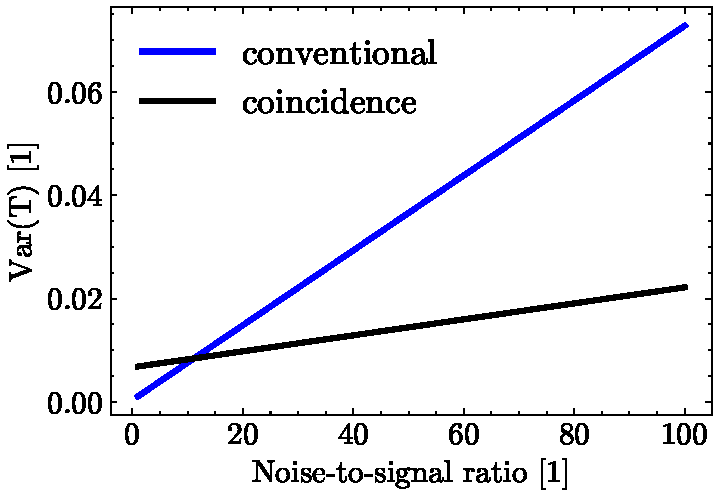
\includegraphics[width=\textwidth]{Images/SimulationSweepSNR_2.pdf}
		\end{minipage}
		\hfill
		\begin{minipage}{.35\textwidth}
			\resizebox{\linewidth}{!}{%
				\begin{tabular}{@{}l@{\hspace{50pt}}lll@{}}
					\toprule[1.5pt]
					\textbf{Parameter} &  \textbf{Value}\\
					\midrule
					$\eta_{\text{idl}}$ (\%) & 0.09 \\
					$\eta_{\text{sig}}$ (\%) & 2.6 \\
					$R_{\text{idl}}$ (kHz) & 10 \\
					\textcolor{red}{$R_{\text{noise,idl}}$ (kHz)} & \textcolor{red}{10 - 1000}\\
					$R_{\text{noise,sig}}$ (Hz)  & 7 \\
					$T$ (1) & 0.9\\
					\bottomrule[1.5pt]
				\end{tabular}
			}
		\end{minipage}
	\end{frame}
	
	
	\begin{frame}{Simulation}
		\begin{minipage}{.55\textwidth}
			\centering
			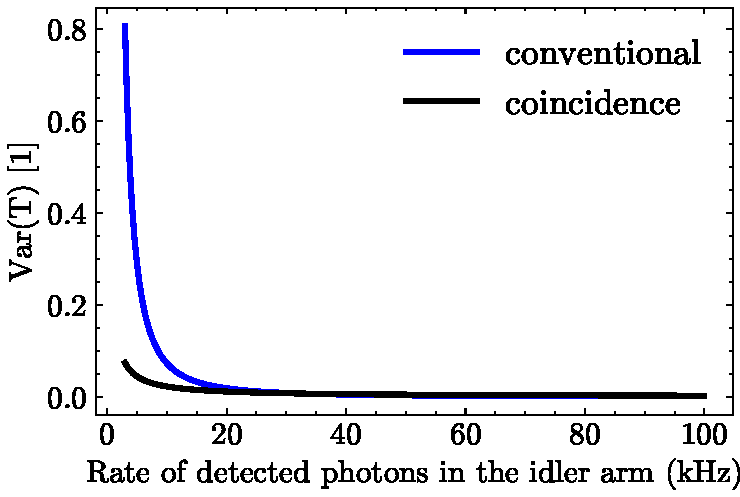
\includegraphics[width=\textwidth]{Images/SimulationSweepRateIdl_2}
		\end{minipage}
		\hfill
		\begin{minipage}{.35\textwidth}
			\resizebox{\linewidth}{!}{%
				\begin{tabular}{@{}l@{\hspace{50pt}}lll@{}}
					\toprule[1.5pt]
					\textbf{Parameter} &  \textbf{Value}\\
					\midrule
					$\eta_{\text{idl}}$ (\%) & 0.09 \\
					$\eta_{\text{sig}}$ (\%) & 2.6 \\
					\textcolor{red}{$R_{\text{idl}}$ (kHz)} & \textcolor{red}{3 - 100} \\
					$R_{\text{noise,idl}}$ (kHz) & 1000\\
					$R_{\text{noise,sig}}$ (Hz)  & 7 \\
					$T$ (1) & 0.9\\
					\bottomrule[1.5pt]
				\end{tabular}
			}
		\end{minipage}
	\end{frame}
	
	\section{Summary}
	
	\begin{frame}{Summary and Outlook}
		\begin{block}{Can coincidence measurements provide more precise results?}
			Achievements:
			\begin{itemize}
				\item Model for variance of transmittance
				\item Experimental verification of photon statistics
				\item Found regions where coincidence approach offers advantages
			\end{itemize}
		\end{block}
		
	\end{frame}
	
	\begin{frame}{Summary and Outlook}
		\begin{Block}{Git repository}
			public accessible:\\
			{\scriptsize\url{https://git.tpi.uni-jena.de/mstnhsr/latexbeamer_corporatedesign}}
		\end{Block}
		\begin{Block}{Feedback}
			marc.steinhauser@uni-jena.de
		\end{Block}
	\end{frame}
	
	
	
	\begin{frame}{Slide title in Palatino Linotype Font}
		\begin{block}{block environment (lower-case b)}
			itemize:
			\begin{itemize}
				\item First Level
				\begin{itemize}
					\item Second Level
					\begin{itemize}
						\item Third Level has no item mark
					\end{itemize}
				\end{itemize}
			\end{itemize}
		\end{block}
		\begin{Block}{Block environment (upper-case B)}
			enumerate:
			\begin{enumerate}
				\item First Level
				\begin{enumerate}
					\item Second Level
					\begin{enumerate}
						\item Third Level
					\end{enumerate}
				\end{enumerate}
			\end{enumerate}
		\end{Block}
	\end{frame}
\end{document}
 
